\documentclass{beamer}

% Theme configuration
\usetheme{Madrid}
\usecolortheme{dolphin}

% Required packages
\usepackage[utf8]{inputenc}
\usepackage[T1]{fontenc}
\usepackage[french]{babel}
\usepackage{graphicx}
\usepackage{booktabs}
\usepackage{amsmath}
\usepackage{hyperref}
\usepackage{xcolor}
\usepackage{listings}

% Custom colors
\definecolor{primary}{RGB}{0,102,204}
\definecolor{secondary}{RGB}{102,102,153}
\definecolor{accent}{RGB}{204,0,0}
\definecolor{codegray}{rgb}{0.5,0.5,0.5}
\definecolor{codepurple}{rgb}{0.58,0,0.82}
\definecolor{codeblue}{rgb}{0,0,0.9}
\definecolor{codegreen}{rgb}{0.1,0.6,0.1}

% Code listing style
\lstdefinestyle{codestyle}{
    basicstyle=\ttfamily\footnotesize,
    numbers=left,
    numberstyle=\tiny\color{codegray},
    stepnumber=1,
    numbersep=5pt,
    backgroundcolor=\color{white!95!black},
    showspaces=false,
    showstringspaces=false,
    showtabs=false,
    frame=tb,
    tabsize=2,
    captionpos=b,
    breaklines=true,
    breakatwhitespace=false,
    stringstyle=\color{codepurple},
    commentstyle=\color{codegreen},
    keywordstyle=\color{codeblue}
}

% Image path configuration
\graphicspath{{week_1_img/}{week_2_img/}{week_3_img/}{week_4_img/}{images/}{./}}

% Title information
\title[Plateforme LearnExpert]{Conception et Développement d'une Plateforme E-learning}
\subtitle{Rapport de Stage - IAAI Academy}
\author[Zakaria el Khaldi]{Zakaria el Khaldi}
\institute[BTS Al-Kendi]{Centre BTS Al-Kendi de Casablanca}
\date{Juin 2025}
\logo{\includegraphics[height=1cm]{LOGO_IAAI.png}}

\begin{document}

\frame{\titlepage}

\begin{frame}
\frametitle{Plan de la Présentation}
\tableofcontents
\end{frame}

% 1. Introduction (2 min)
\section{Introduction}

\begin{frame}
\frametitle{Présentation du Projet}
\begin{itemize}
    \item \textbf{Contexte} : Stage de fin d'études de 4 semaines à IAAI Academy
    \item \textbf{Projet} : Plateforme e-learning LearnExpert
    \item \textbf{Objectif} : Développement d'une solution d'apprentissage interactive pour la programmation et les technologies web
\end{itemize}
\begin{center}
    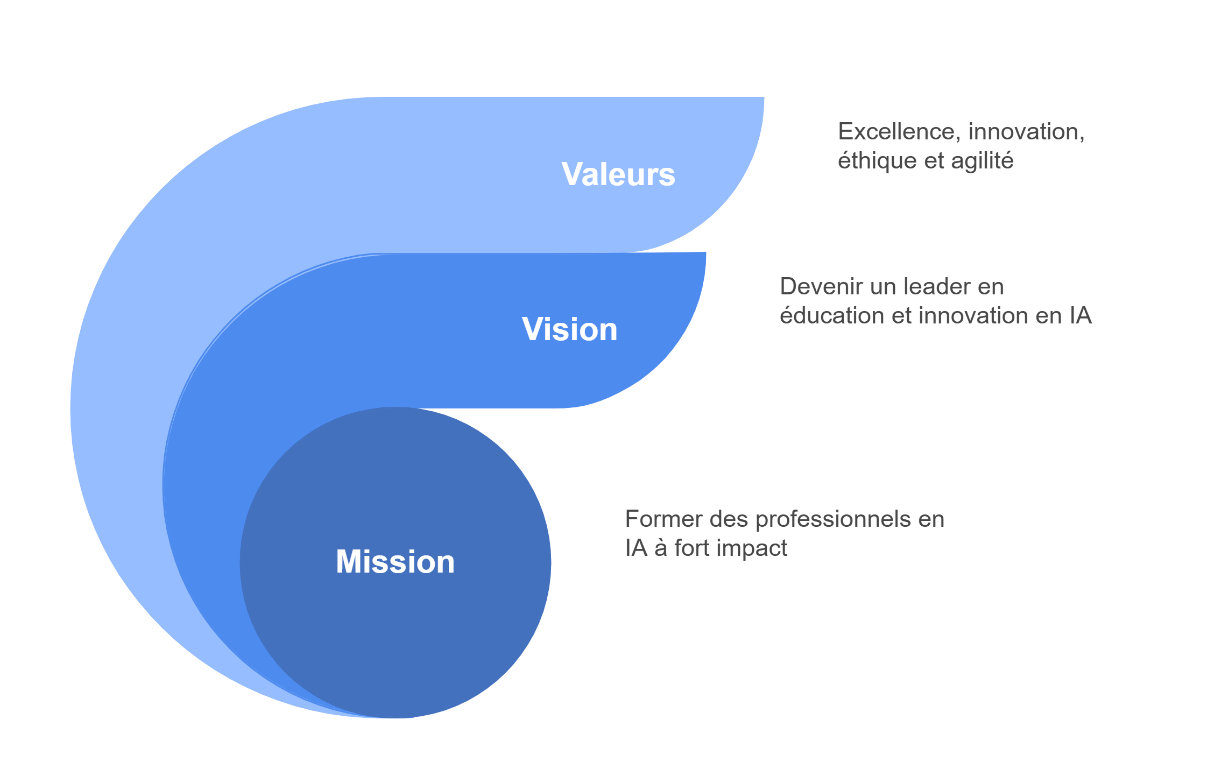
\includegraphics[width=0.5\textwidth]{images/mession.png}
\end{center}
\end{frame}

\begin{frame}
\frametitle{Problématique et Objectifs}
\begin{columns}
\column{0.5\textwidth}
\textbf{Problématiques identifiées :}
\begin{itemize}
    \item Contenu générique des plateformes actuelles
    \item Manque d'interactivité pour l'apprentissage de la programmation
    \item Fragmentation des ressources éducatives
    \item Absence de personnalisation
\end{itemize}

\column{0.5\textwidth}
\textbf{Objectifs du projet :}
\begin{itemize}
    \item Approche centrée sur la pratique
    \item Personnalisation via l'IA
    \item Intégration de contenus structurés
    \item Architecture évolutive
    \item Expérience utilisateur engageante
\end{itemize}
\end{columns}
\end{frame}

% 2. Methodology (2 min)
\section{Méthodologie}

\begin{frame}
\frametitle{Approche de Développement}
\begin{columns}
\column{0.5\textwidth}
\textbf{Méthodologie adoptée :}
\begin{itemize}
    \item Approche en cascade adaptée
    \item Phases structurées
    \item Revues itératives
    \item Développement incrémental
\end{itemize}

\column{0.5\textwidth}
\textbf{Outils de modélisation :}
\begin{itemize}
    \item UML (Unified Modeling Language)
    \item Diagrammes de cas d'utilisation
    \item Diagrammes de séquence
    \item Diagrammes de classes
    \item Modèles de données
\end{itemize}
\end{columns}
\end{frame}

\begin{frame}
\frametitle{Planification du Projet}
\begin{itemize}
    \item \textbf{Diagramme PERT} : Visualisation des dépendances entre tâches
    \item \textbf{Diagramme de Gantt} : Organisation temporelle
    \item \textbf{Chemin critique} : Identification des tâches prioritaires
\end{itemize}
\begin{center}
    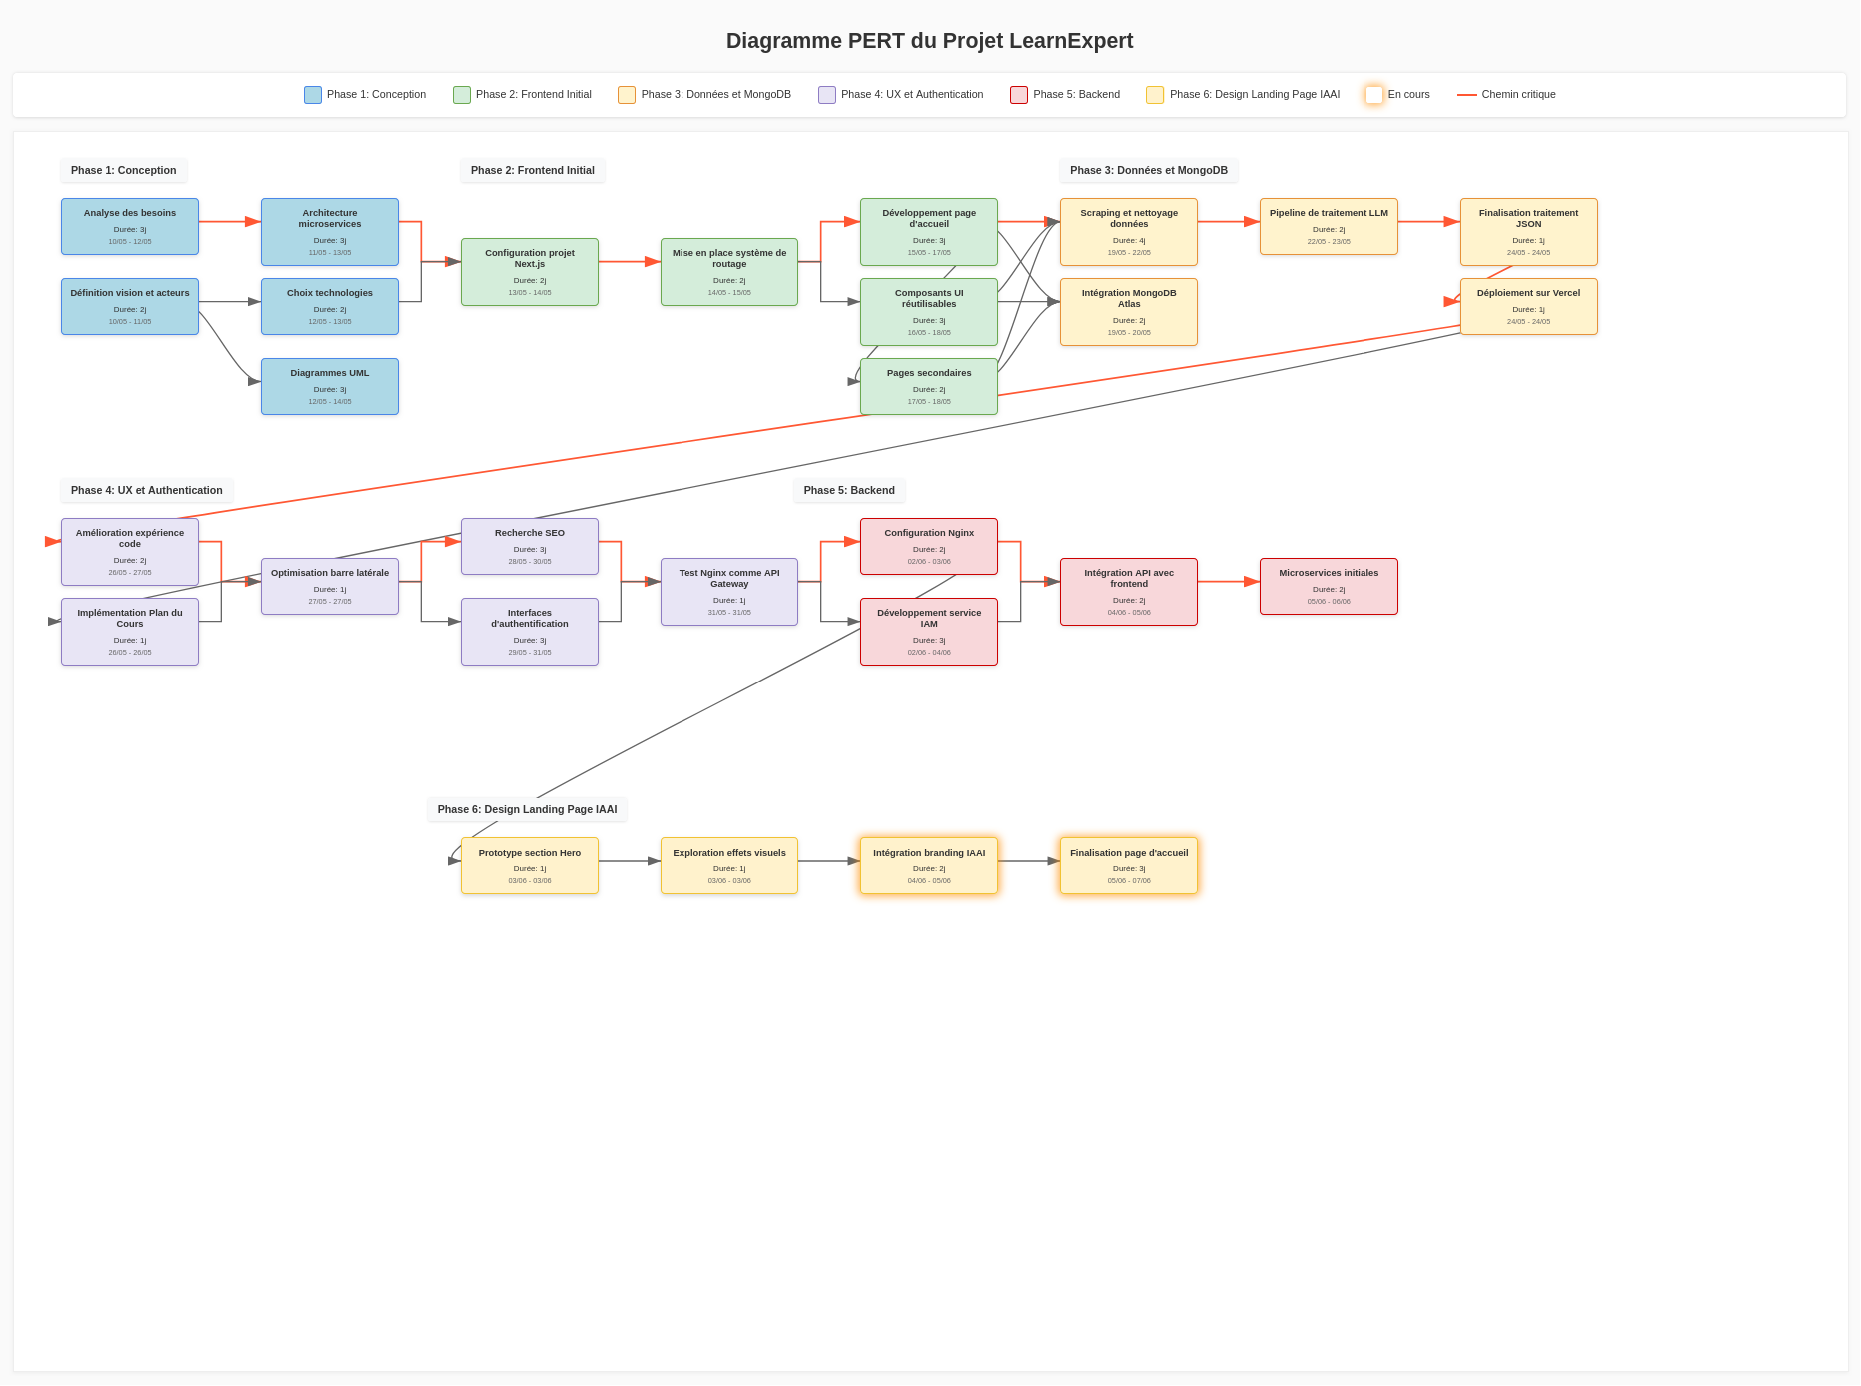
\includegraphics[width=0.8\textwidth,height=4.5cm,keepaspectratio]{images/gestion_projet/pert_diagram.png}
\end{center}
\end{frame}

% 3. System Architecture (4 min)
\section{Architecture du Système}

\begin{frame}
\frametitle{Vue d'Ensemble de l'Architecture}
\begin{center}
    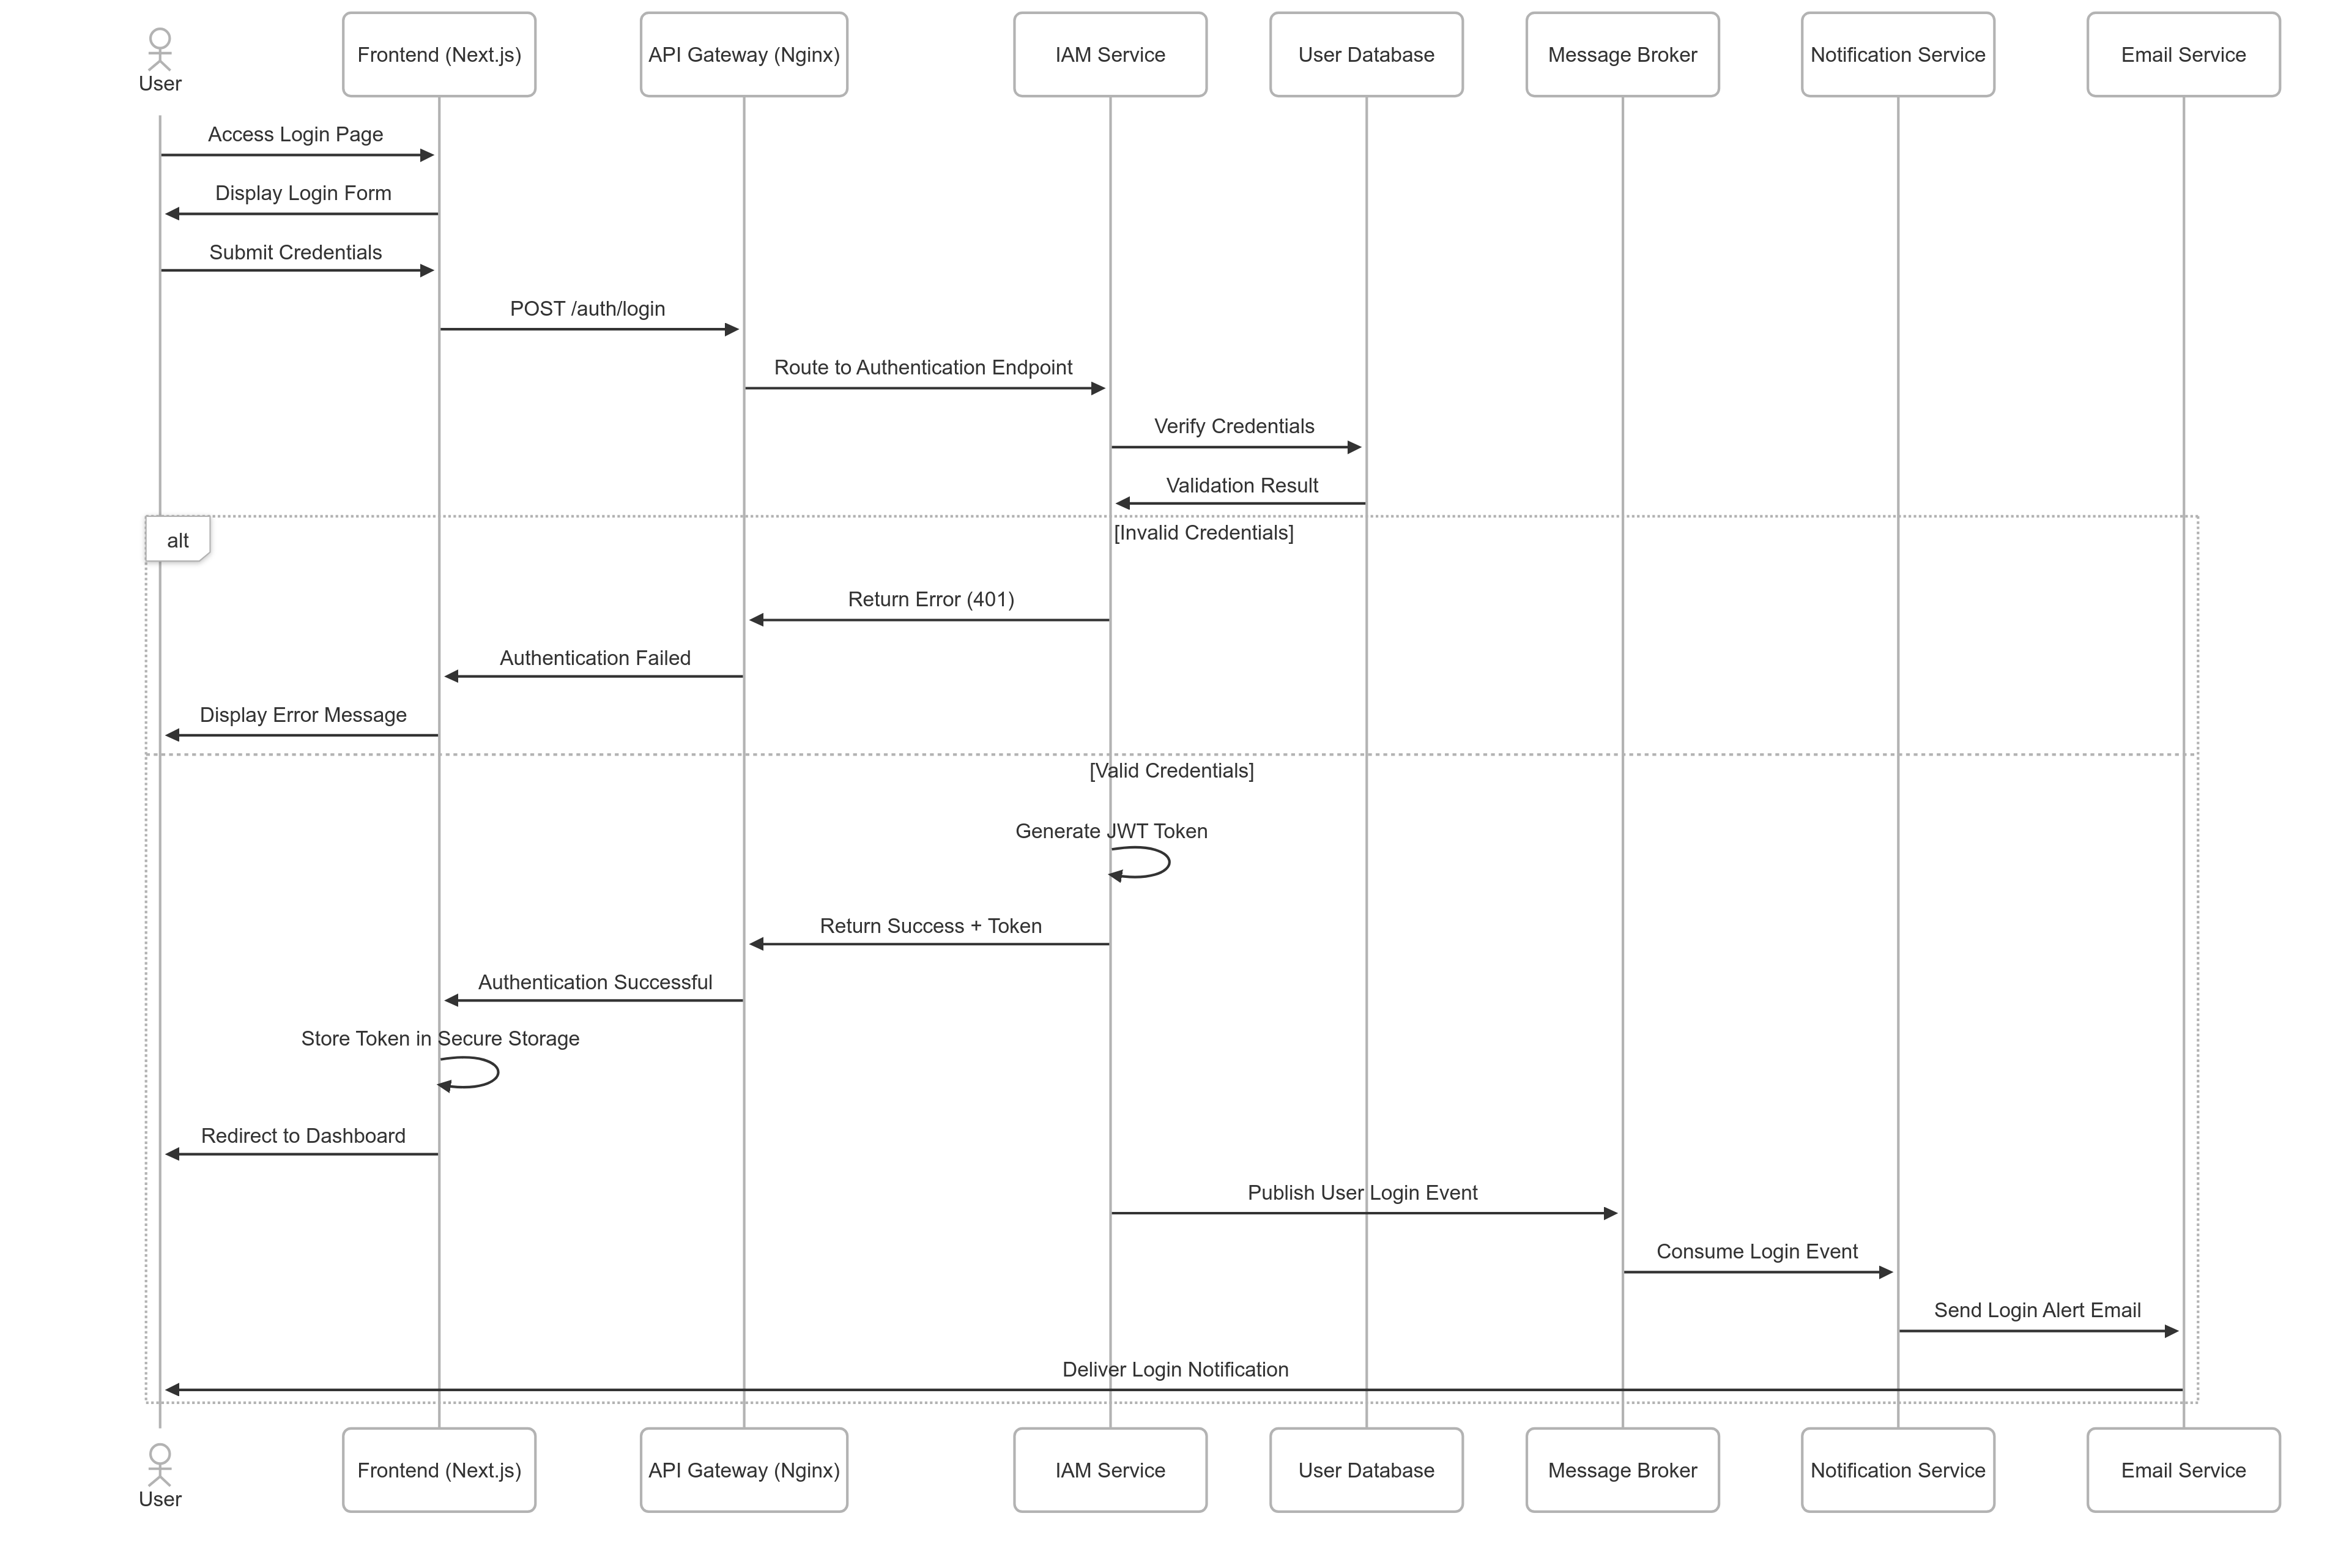
\includegraphics[width=0.9\textwidth,height=6cm,keepaspectratio]{Editor _ Mermaid Chart-2025-06-06-214630.png}
\end{center}
\end{frame}

\begin{frame}
\frametitle{Architecture Microservices}
\begin{columns}
\column{0.5\textwidth}
\textbf{Avantages de l'approche microservices :}
\begin{itemize}
    \item Scalabilité indépendante des services
    \item Maintenabilité facilitée
    \item Résilience accrue
    \item Flexibilité technologique
\end{itemize}

\column{0.5\textwidth}
\textbf{Services principaux :}
\begin{itemize}
    \item Service IAM
    \item Service de Contenu
    \item Service de Facturation
    \item Service de Certification
    \item Service d'Analytique
    \item Service de Notification
\end{itemize}
\end{columns}

\vspace{0.3cm}
\begin{center}
    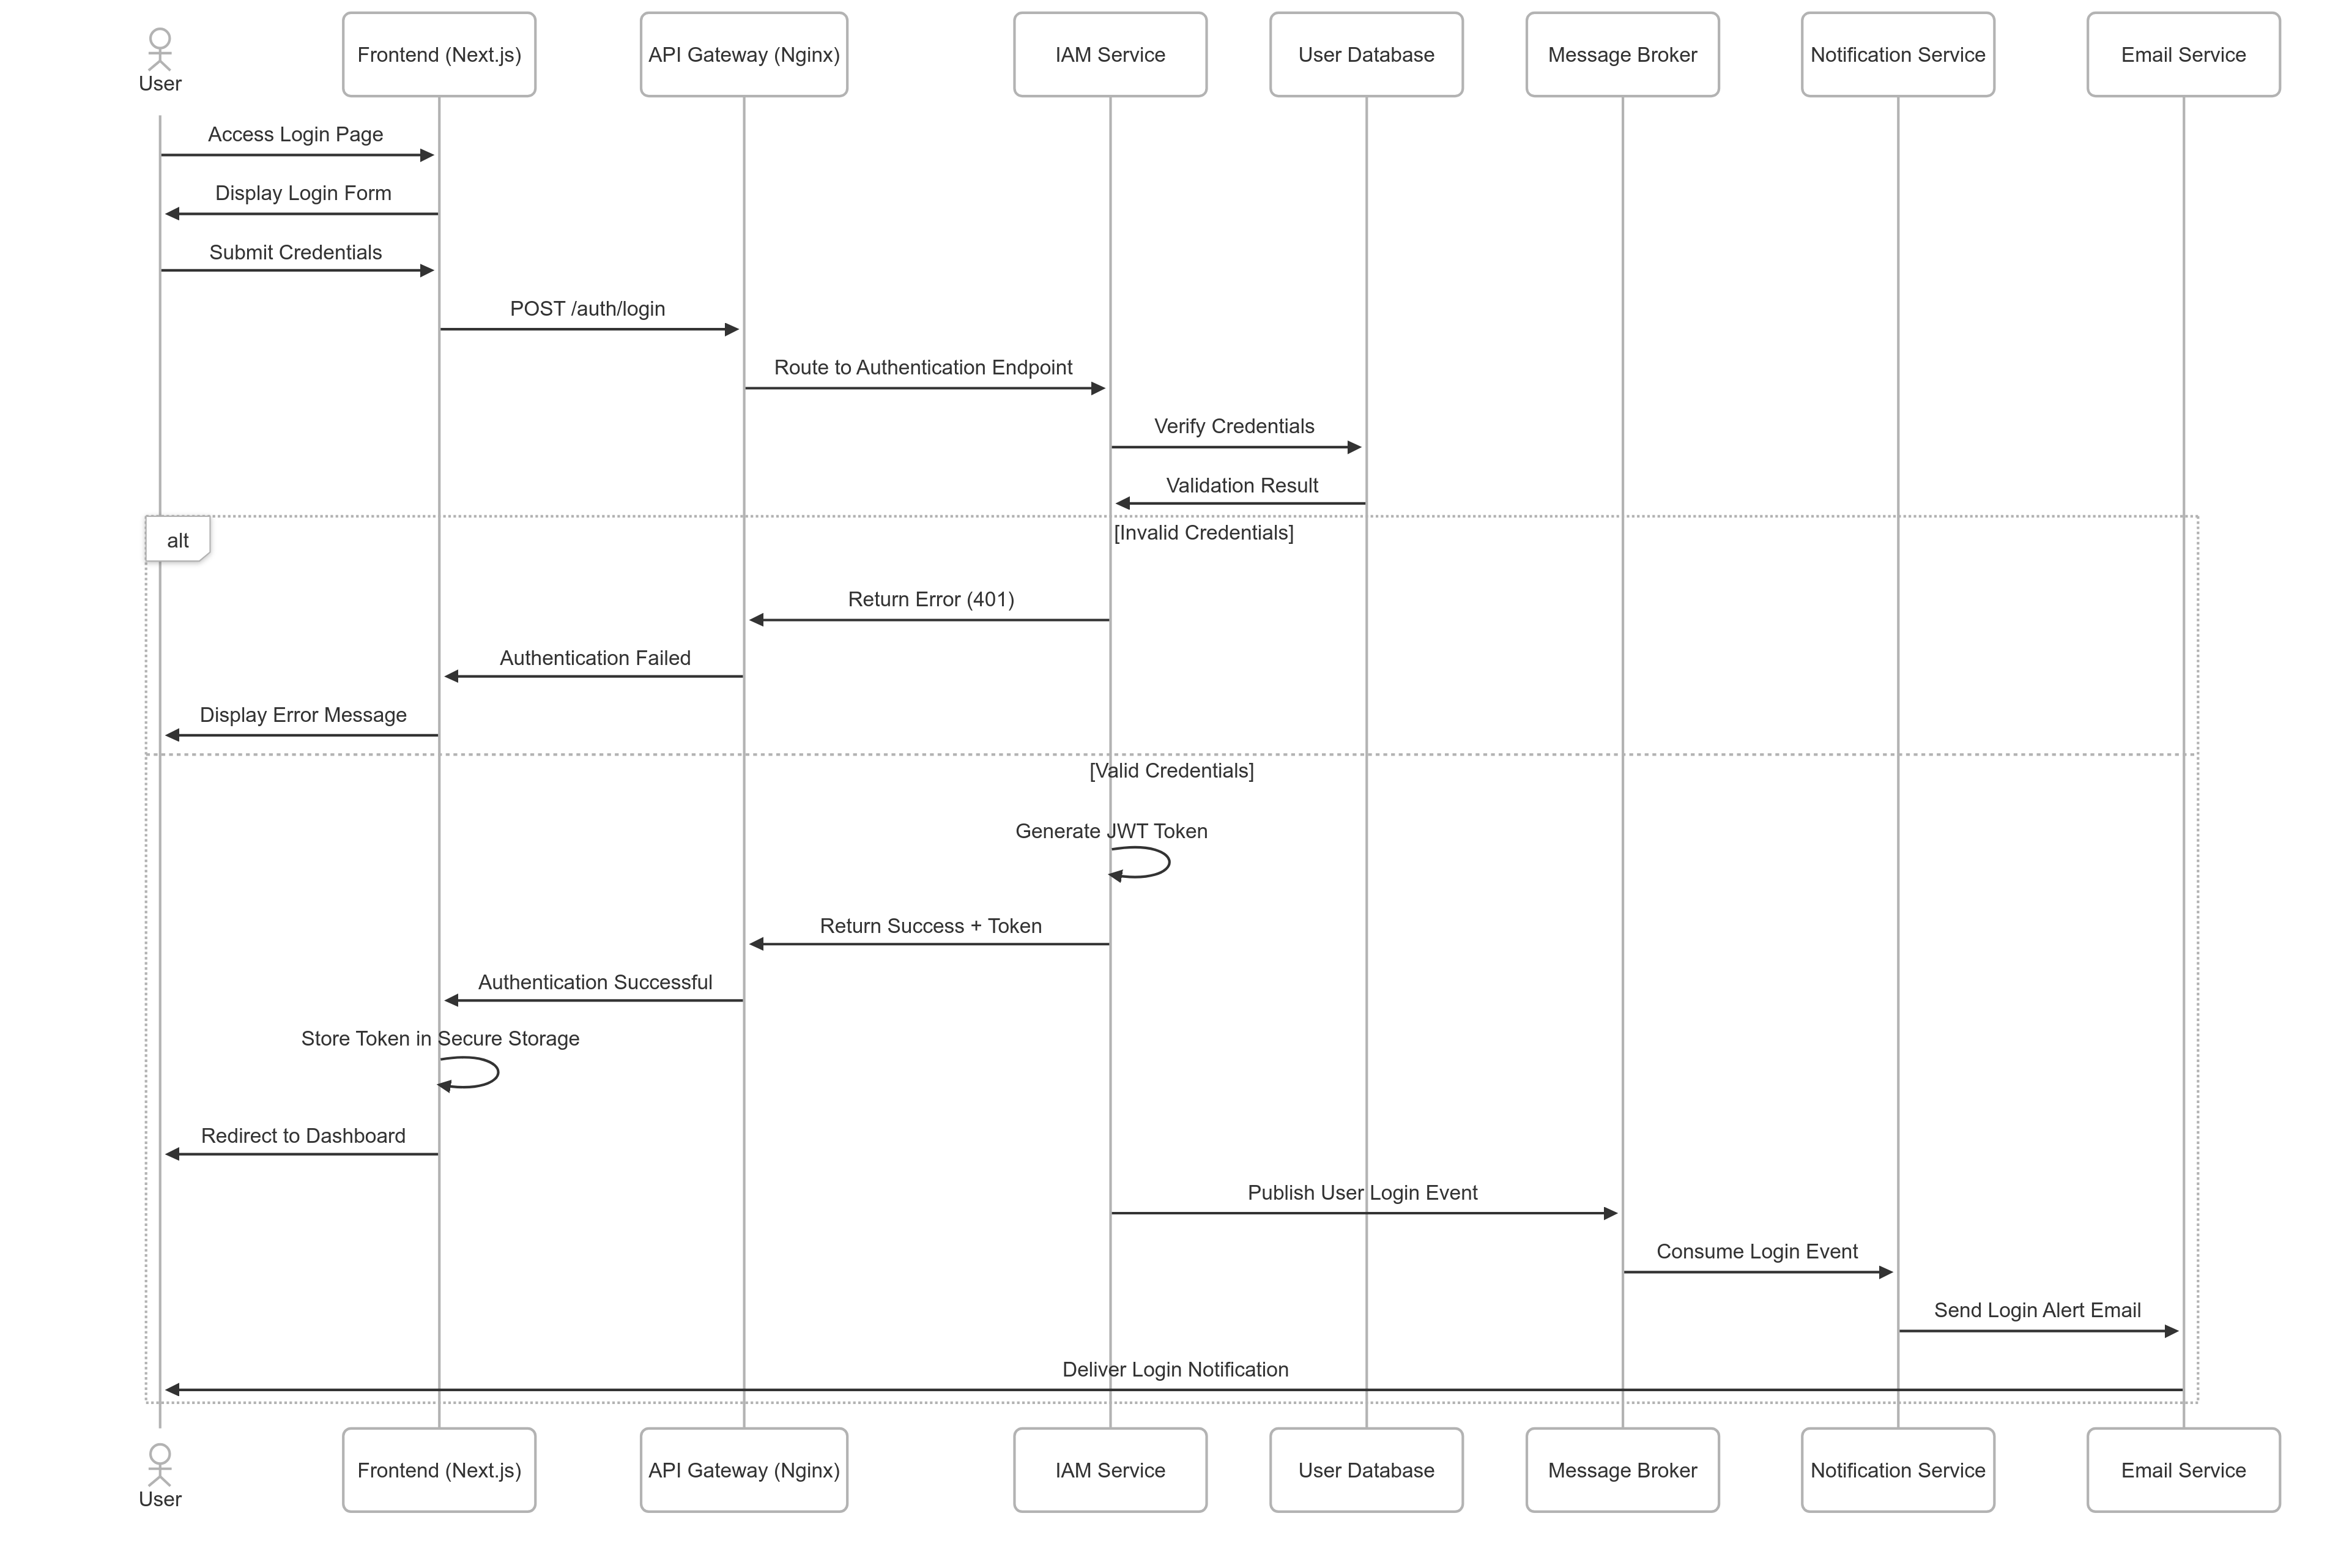
\includegraphics[width=0.8\textwidth,height=3.5cm,keepaspectratio]{images/sequence_diagram.png}
\end{center}
\end{frame}

\begin{frame}
\frametitle{Technologies Frontend}
\begin{columns}
\column{0.5\textwidth}
\textbf{Framework et langages :}
\begin{itemize}
    \item Next.js (React)
    \item TypeScript
    \item Tailwind CSS
    \item Framer Motion
\end{itemize}

\column{0.5\textwidth}
\textbf{Outils spécialisés :}
\begin{itemize}
    \item Monaco Editor (éditeur de code)
    \item React Hook Form (gestion des formulaires)
    \item Radix UI (composants accessibles)
\end{itemize}
\end{columns}
\begin{center}
    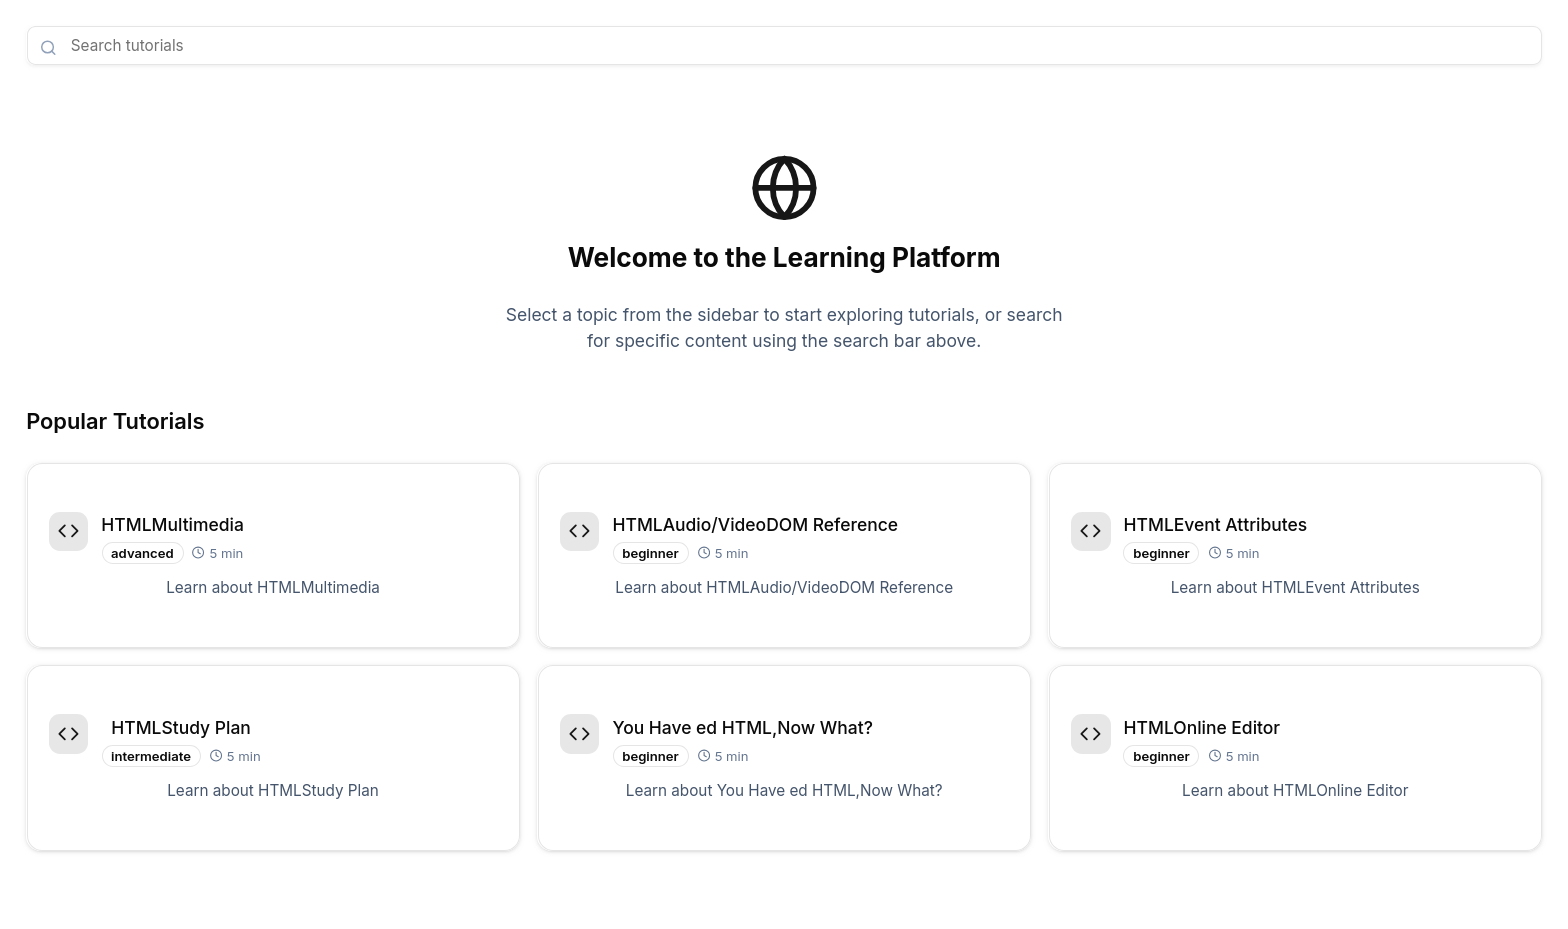
\includegraphics[width=0.5\textwidth]{week_3_img/accueil.png}
\end{center}
\end{frame}

\begin{frame}
\frametitle{Technologies Backend}
\begin{columns}
\column{0.5\textwidth}
\textbf{Langages et frameworks :}
\begin{itemize}
    \item Node.js avec Express
    \item Python avec FastAPI
    \item Go (pour services critiques)
\end{itemize}

\column{0.5\textwidth}
\textbf{Infrastructure :}
\begin{itemize}
    \item Nginx (API Gateway)
    \item MongoDB (données non-structurées)
    \item PostgreSQL/Supabase (données relationnelles)
    \item Docker (conteneurisation)
    \item Apache Kafka (communication event-driven)
\end{itemize}
\end{columns}
\end{frame}

\begin{frame}
\frametitle{Conception des Bases de Données}
\begin{columns}
\column{0.48\textwidth}
\textbf{Modèle IAM :}
\begin{center}
    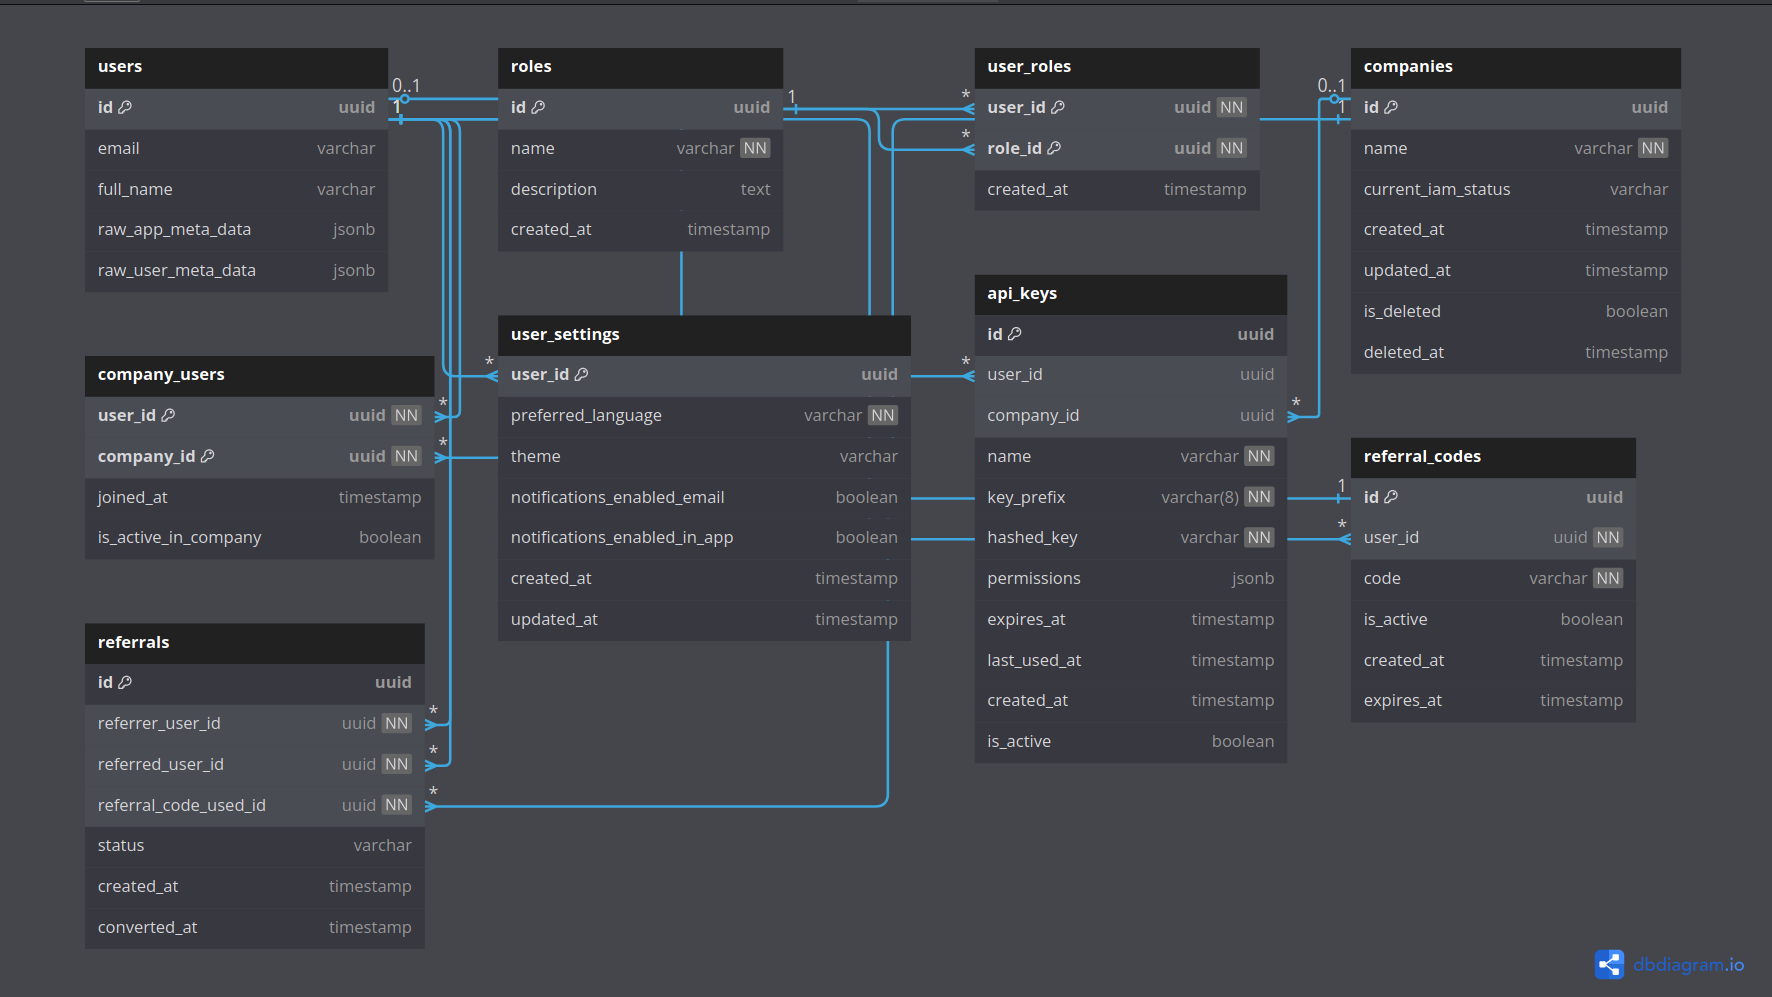
\includegraphics[width=\textwidth,height=5cm,keepaspectratio]{week_1_img/services_db_screanshots/Screenshot 2025-06-06 at 15-08-36 IAM_Service.pdf.png}
\end{center}

\column{0.48\textwidth}
\textbf{Modèle de Contenu :}
\begin{center}
    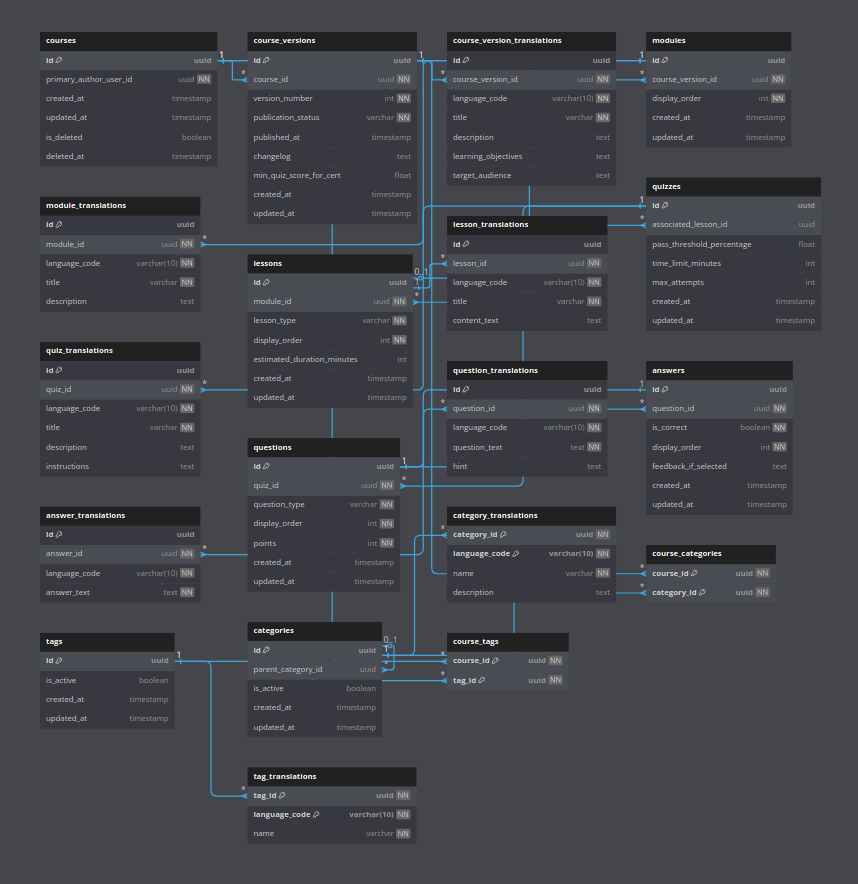
\includegraphics[width=\textwidth,height=5cm,keepaspectratio]{week_1_img/services_db_screanshots/Screenshot 2025-06-06 at 15-07-51 Content_Service.pdf.png}
\end{center}
\end{columns}
\end{frame}

% 4. Key Features & Functionality (4 min)
\section{Fonctionnalités Principales}

\begin{frame}
\frametitle{Système de Gestion des Utilisateurs}
\begin{itemize}
    \item \textbf{Authentification multi-niveaux}
    \begin{itemize}
        \item Inscription et connexion sécurisées
        \item Vérification par email
        \item Récupération de mot de passe
    \end{itemize}
    \item \textbf{Gestion des rôles}
    \begin{itemize}
        \item Apprenant individuel
        \item Employé d'entreprise
        \item Administrateur d'entreprise
        \item Créateur de cours
        \item Consultant
        \item Agent de support
        \item Administrateur de plateforme
    \end{itemize}
    \item \textbf{Personnalisation du profil}
    \item \textbf{Paramètres de confidentialité et de notification}
\end{itemize}
\end{frame}

\begin{frame}
\frametitle{Gestion des Cours}
\begin{columns}
\column{0.48\textwidth}
\textbf{Organisation du contenu :}
\begin{itemize}
    \item Structure hiérarchique
    \item Multi-formats (texte, code, vidéo)
    \item Métadonnées avancées
    \item Versionnement
\end{itemize}

\column{0.48\textwidth}
\textbf{Interface d'apprentissage :}
\begin{itemize}
    \item Contenu théorique structuré
    \item Exercices pratiques intégrés
    \item Navigation intuitive
    \item Mode sombre/clair
\end{itemize}
\end{columns}

\vspace{0.3cm}
\begin{center}
    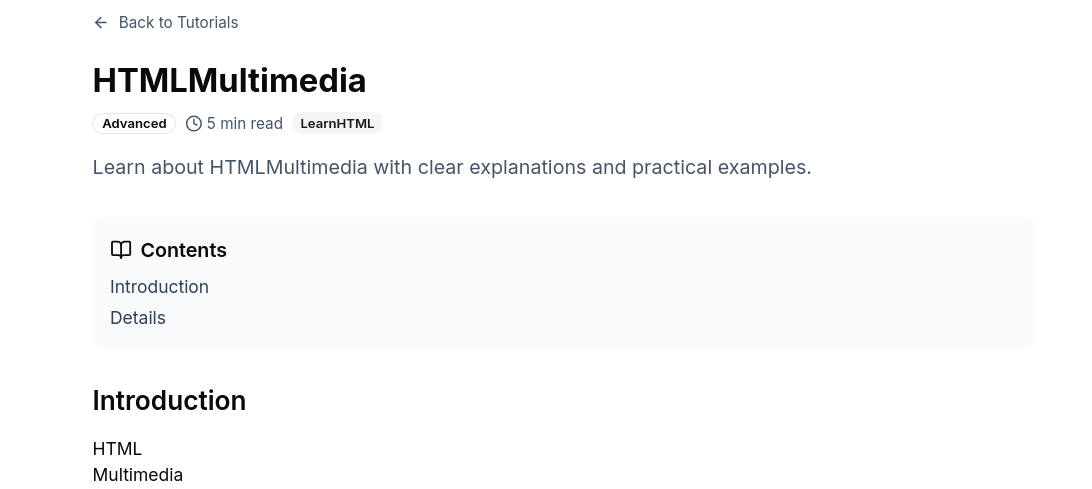
\includegraphics[width=0.65\textwidth,height=4cm,keepaspectratio]{week_3_img/part1.png}
\end{center}
\end{frame}

\begin{frame}
\frametitle{Parcours d'Apprentissage}
\begin{columns}
\column{0.55\textwidth}
\textbf{Parcours thématiques spécialisés :}
\begin{itemize}
    \item Intelligence Artificielle
    \item Cybersécurité
    \item Compétences IT
    \item Préparation aux entretiens
\end{itemize}
\textbf{Caractéristiques :}
\begin{itemize}
    \item Personnalisation intelligente
    \item Progression structurée
    \item Tableau de bord adaptatif
\end{itemize}

\column{0.42\textwidth}
\begin{center}
    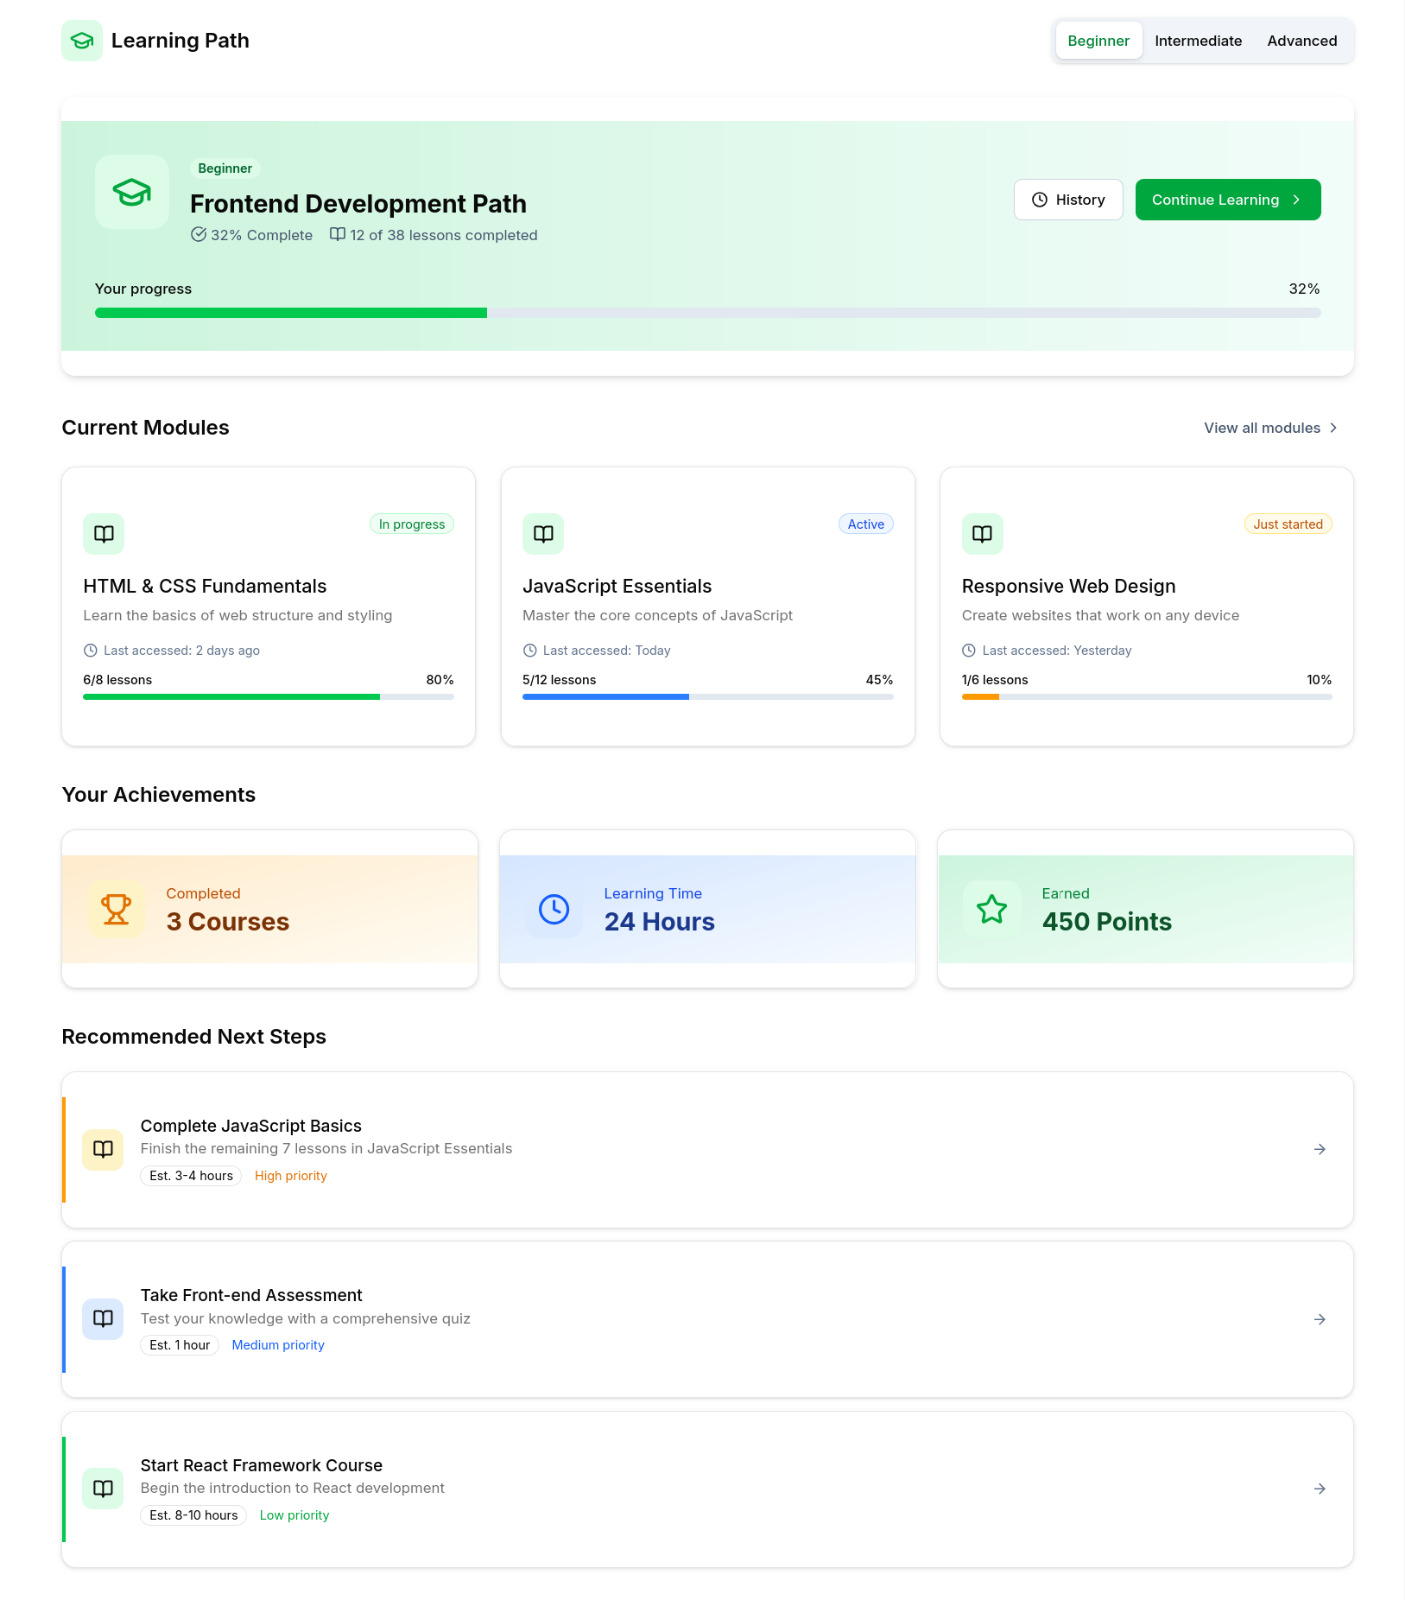
\includegraphics[width=\textwidth,height=5cm,keepaspectratio]{old-reports/week_4_img/learnpath.jpeg}
\end{center}
\end{columns}
\end{frame}

\begin{frame}
\frametitle{Évaluation et Certification}
\begin{columns}
\column{0.5\textwidth}
\textbf{Systèmes d'évaluation :}
\begin{itemize}
    \item Quiz interactifs
    \item Exercices de code avec vérification
    \item Retour personnalisé
    \item Projets pratiques
\end{itemize}

\column{0.46\textwidth}
\begin{center}
    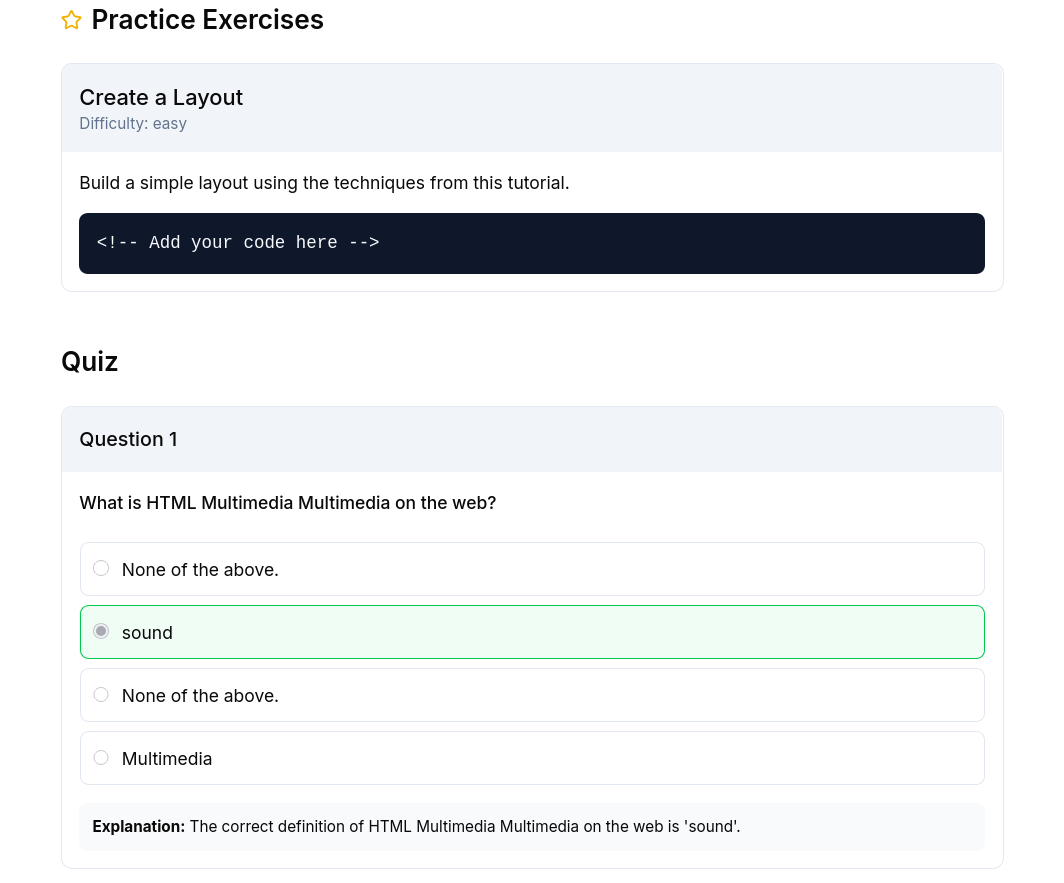
\includegraphics[width=\textwidth,height=4.5cm,keepaspectratio]{week_3_img/part2.png}
\end{center}
\end{columns}

\vspace{0.3cm}
\textbf{Certification :}
\begin{itemize}
    \item Badges et récompenses pour motiver les apprenants
    \item Certificats d'achèvement vérifiables
    \item Intégration avec les réseaux professionnels
\end{itemize}
\end{frame}

% 5. Implementation Highlights (3 min)
\section{Points Forts de l'Implémentation}

\begin{frame}
\frametitle{Défis Techniques}
\begin{itemize}
    \item \textbf{Traitement des données de contenu}
    \begin{itemize}
        \item Difficulté à séparer automatiquement le contenu explicatif du code
        \item Approches conventionnelles limitées à 80\% de précision
        \item Volume important de données à traiter (70+ cours)
    \end{itemize}
    \item \textbf{Performance de l'éditeur de code}
    \begin{itemize}
        \item Intégration complexe de Monaco Editor
        \item Exécution sécurisée du code utilisateur
        \item Optimisation pour appareils mobiles
    \end{itemize}
    \item \textbf{Interfaces riches et complexes}
    \begin{itemize}
        \item Animations fluides sans impact sur les performances
        \item Gestion des composants UI dynamiques
        \item Optimisation du chargement
    \end{itemize}
\end{itemize}
\end{frame}

\begin{frame}
\frametitle{Solutions Implémentées}
\begin{columns}
\column{0.48\textwidth}
\textbf{Pipeline de traitement LLM :}
\begin{itemize}
    \item Modèles LLM en parallèle
    \item Traitement asynchrone
    \item Segmentation intelligente
    \item Réduction temps: 15h → 7-8h
    \item Précision proche de 100\%
\end{itemize}

\column{0.48\textwidth}
\textbf{Éditeur de code interactif :}
\begin{itemize}
    \item Coloration syntaxique (6+ langages)
    \item Exécution en temps réel
    \item Dispositions personnalisables
    \item Thèmes adaptables
    \item Mode plein écran
\end{itemize}
\end{columns}

\vspace{0.3cm}
\begin{center}
    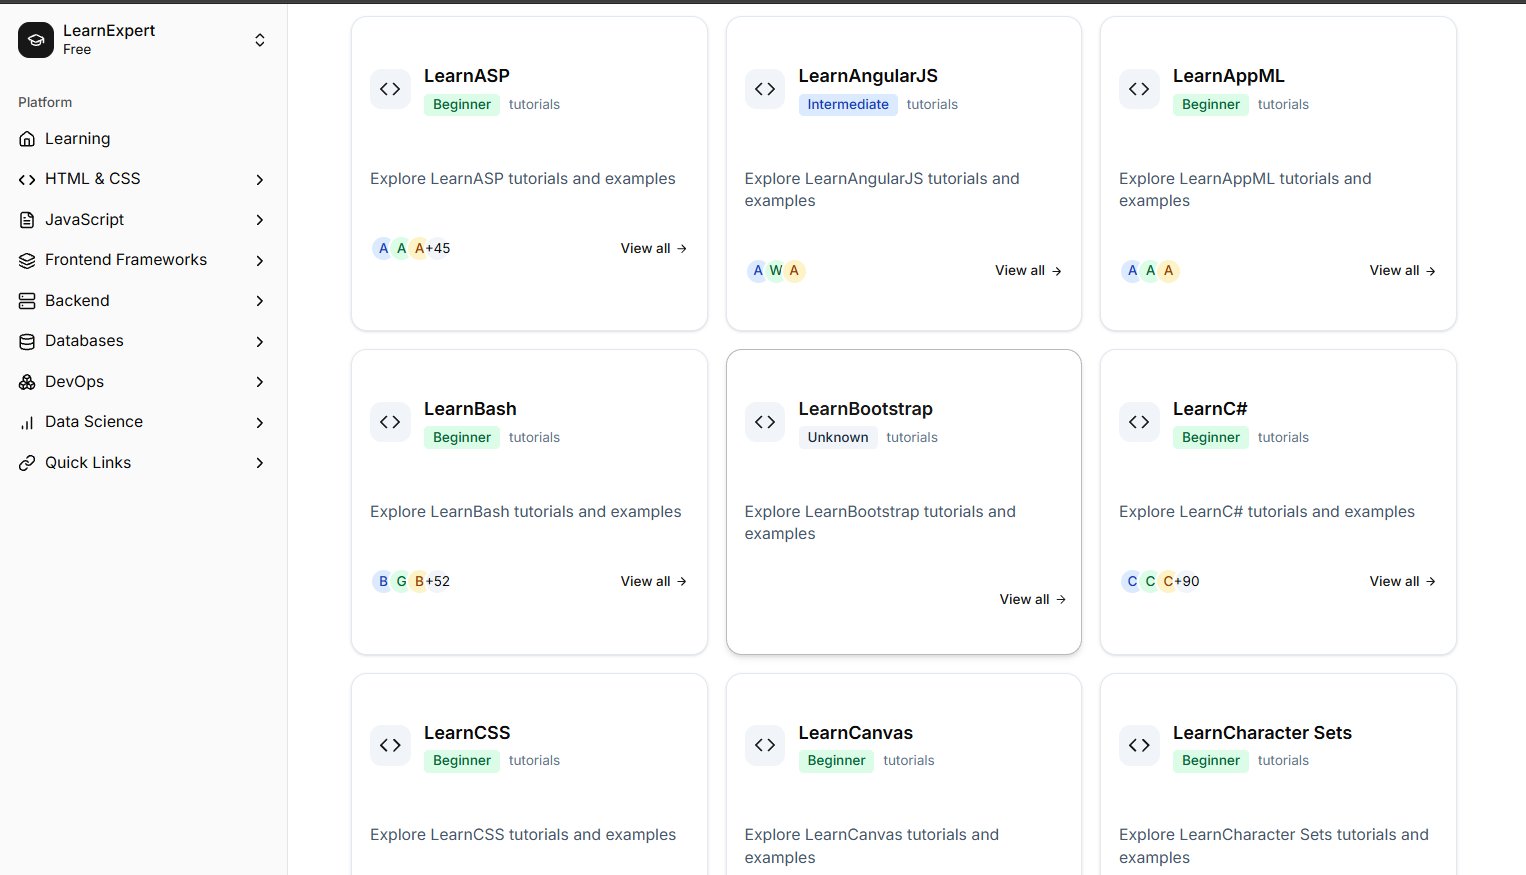
\includegraphics[width=0.6\textwidth,height=3.3cm,keepaspectratio]{week_3_img/Screenshot 2025-05-20 164411.png}
\end{center}
\end{frame}

\begin{frame}
\frametitle{Optimisations de Performance}
\begin{itemize}
    \item \textbf{Frontend}
    \begin{itemize}
        \item Code splitting et lazy loading des composants
        \item Optimisation automatique des images
        \item Préchargement intelligent des ressources
        \item Mise en cache sélective
    \end{itemize}
    \item \textbf{Backend}
    \begin{itemize}
        \item Indexation optimisée des bases de données
        \item Mise en cache des requêtes fréquentes
        \item API Gateway avec distribution de charge
        \item Compression des réponses
    \end{itemize}
    \item \textbf{Infrastructure}
    \begin{itemize}
        \item Déploiement sur Vercel pour le frontend
        \item Containerisation Docker pour les services backend
        \item Configuration optimisée de Nginx
    \end{itemize}
\end{itemize}
\end{frame}

% 6. Project Timeline (2 min)
\section{Calendrier du Projet}

\begin{frame}
\frametitle{Diagramme de Gantt}
\begin{center}
    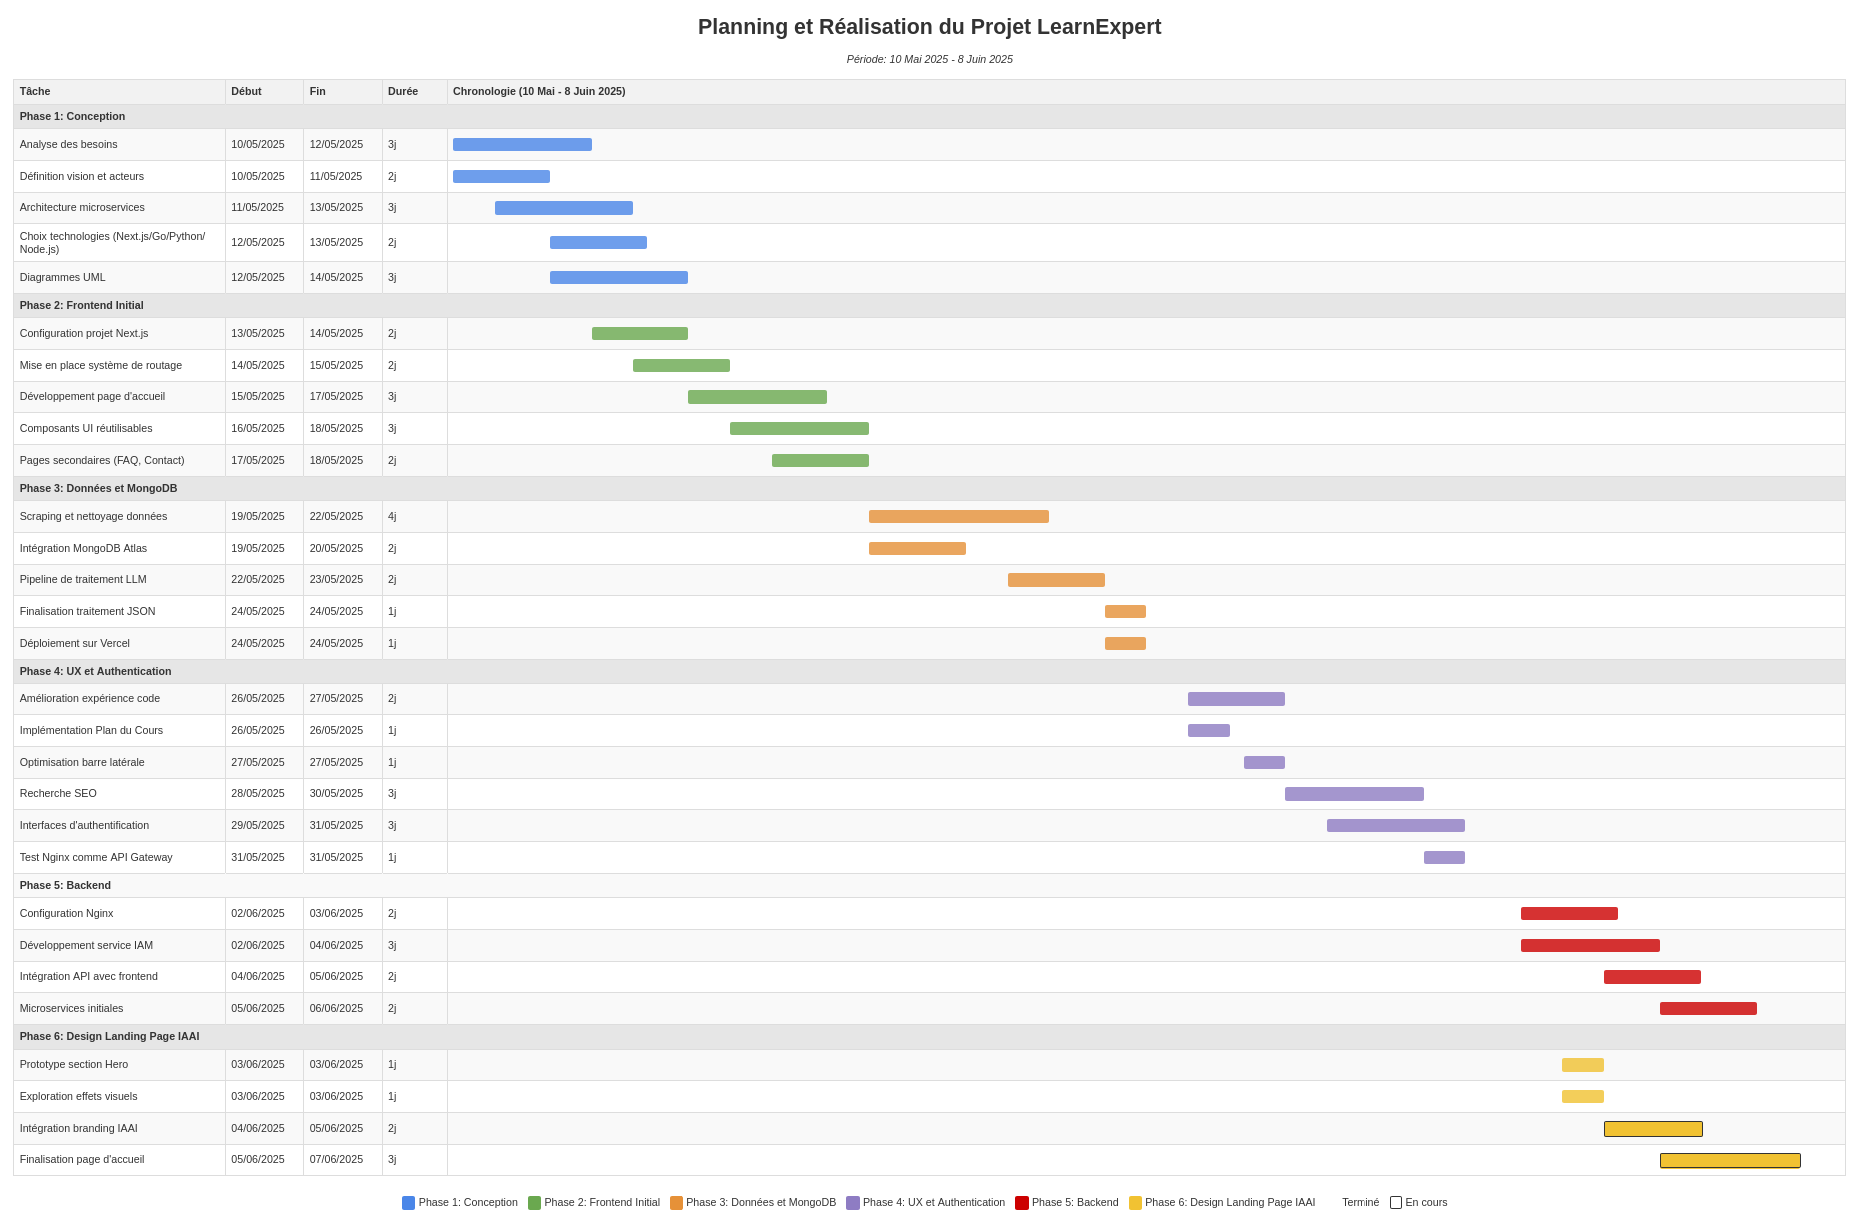
\includegraphics[width=0.95\textwidth,height=7cm,keepaspectratio]{Screenshot 2025-06-08 at 20-35-06 Planning du Projet LearnExpert - Diagramme de Gantt.png}
\end{center}
\end{frame}

\begin{frame}
\frametitle{Analyse du Chemin Critique}
\begin{itemize}
    \item \textbf{Phases critiques identifiées :}
    \begin{itemize}
        \item Conception initiale
        \item Développement du frontend principal
        \item Implémentation des pages secondaires
        \item Services backend essentiels
    \end{itemize}
    \item \textbf{Parallélisation effective :}
    \begin{itemize}
        \item Développement UI et système de routage
        \item Backend et traitement des données
        \item Design et intégration frontend
    \end{itemize}
    \item \textbf{Répartition équilibrée :} 4 semaines divisées en phases logiques
\end{itemize}
\end{frame}

% 7. Conclusion & Future Work (2 min)
\section{Conclusion et Perspectives}

\begin{frame}
\frametitle{Résultats du Projet}
\begin{columns}
\column{0.5\textwidth}
\textbf{Réalisations principales :}
\begin{itemize}
    \item Architecture microservices fonctionnelle
    \item Interface utilisateur intuitive et responsive
    \item Éditeur de code interactif
    \item Pipeline de traitement de données optimisé
    \item Système d'authentification sécurisé
\end{itemize}

\column{0.5\textwidth}
\textbf{Compétences acquises :}
\begin{itemize}
    \item Maîtrise de Next.js et React
    \item Expérience avec l'architecture microservices
    \item Utilisation avancée de MongoDB et Supabase
    \item Intégration de modèles LLM
    \item Développement agile en contexte réel
\end{itemize}
\end{columns}
\end{frame}

\begin{frame}
\frametitle{Perspectives et Améliorations Futures}
\begin{itemize}
    \item \textbf{Pour IAAI :}
    \begin{itemize}
        \item Enrichissement des fonctionnalités d'IA pour personnaliser les parcours
        \item Analyse avancée des performances des apprenants
        \item Génération de contenu adaptatif
    \end{itemize}
    \item \textbf{Développements techniques envisagés :}
    \begin{itemize}
        \item Application mobile native
        \item Intégration avec des plateformes tierces
        \item Expansion multilingue
        \item Fonctionnalités collaboratives
    \end{itemize}
    \item \textbf{Prochaines étapes :}
    \begin{itemize}
        \item Lancement de la version bêta
        \item Tests utilisateurs à grande échelle
        \item Optimisation continue basée sur les retours
    \end{itemize}
\end{itemize}
\end{frame}

\begin{frame}
\frametitle{Questions ?}
\begin{center}
    \LARGE Merci pour votre attention !\\
    \vspace{1cm}
    Questions ?
\end{center}
\end{frame}

\end{document} 